\documentclass[xcolor=svgnames, 10pt, handout]{beamer}

\usepackage[utf8]{inputenc}
\usepackage[T1]{fontenc}
\usepackage[english]{babel}

%\usepackage{verbatim}

\usepackage[export]{adjustbox}

\usepackage{
    amsmath,
    amsfonts,
    etex,
    fancyvrb,
    graphicx,
    multicol,
    pifont,
    setspace,
    soul,
    spverbatim,
    textcomp,
    xcolor,
    xspace
}

\usepackage{tikz}
\usetikzlibrary{shadows}

%%%SETUP%%%
\hypersetup{
     colorlinks = true,
     linkcolor = blue,
     anchorcolor = blue,
     citecolor = blue,
     filecolor = blue,
     urlcolor = blue
     }
     
%%%THEOREMS%%%
\theoremstyle{example}
\newtheorem*{exercise}{Exercise}
\newtheorem*{question}{Question}
\newtheorem*{answer}{\emph{Answer}}
\newtheorem*{notation}{Notation}

%%%TWEAKS%%%
\setlength\arraycolsep{4pt}
\addtolength\fboxsep{10pt}
\setstretch{1.4}
\setbeamersize{description width=3em}
\setbeamersize{text margin left=.5cm,text margin right=.5cm} 
\renewcommand{\emph}{\alert}
\renewcommand{\arraystretch}{1.2}
\renewcommand{\tabcolsep}{4pt}
\setbeamercolor{alerted text}{fg=magenta}


\graphicspath{{img/}}

%for straight quotes in verbatim:
\usepackage{upquote,textcomp}

%turn off navigation symbols
\beamertemplatenavigationsymbolsempty
\setbeamertemplate{footline}[frame number]

%title page

\author
  [Dr.\ Irene Vrbik]
  {Dr.\ Irene Vrbik}

\date
  {}

\institute
  {University of British Columbia Okanagan \newline \texttt{irene.vrbik@ubc.ca}}
  
\definecolor{iyellow}{RGB}{255, 162, 23}
\definecolor{sgreen}{RGB}{118, 191, 138}

\newcommand{\yellow}[1]{\textcolor{iyellow}{#1}}
\newcommand{\red}[1]{\textcolor{red}{#1}}
\newcommand{\green}[1]{\textcolor{ForestGreen}{#1}}
\newcommand{\blue}[1]{{\textcolor{blue}{#1}}}
\newcommand{\orange}[1]{{\textcolor{orange}{#1}}}
\newcommand{\bblue}[1]{\textcolor{SteelBlue!90!gray}{#1}} % beamer blue
\newcommand{\purple}[1]{{\textcolor{purple}{#1}}}

\newcommand{\el}{\\[1em]\pause}
\newcommand{\nl}{\\[1em]}
\newcommand{\define}[1]{\textbf{\textcolor{orange}{#1}}}

%\newcommand{\answer}[1]{\textit{\textbf{\textcolor{iyellow}{#1}}}}

\newcommand{\command}[1]{\texttt{\textbf{\textcolor{DarkMagenta}{#1}}}}
\newcommand{\ipic}[2]{\includegraphics[width={#2}\textwidth]{#1}}
\newcommand{\cell}[1]{{\sf \textbf{\textcolor{DarkMagenta}{#1}}}}
\newcommand{\ra}{$\rightarrow$}

\newcommand{\ft}[1]{\frametitle{#1}}


\newenvironment{allintypewriter}{\ttfamily}{\par}
\newcommand{\bs}{$\backslash$}

\newcommand*\keystroke[1]{%
  \tikz[baseline=(key.base)]
    \node[%
      draw,
      fill=white,
      drop shadow={shadow xshift=0.25ex,shadow yshift=-0.25ex,fill=black,opacity=0.75},
      rectangle,
      rounded corners=2pt,
      inner sep=1pt,
      line width=0.5pt,
      font=\scriptsize\sffamily
    ](key) {#1\strut}
  ;
}

% timed answer
\newcommand{\tans}[2]{\textbf<#1>{\textit<#1>{{\color<#1>{iyellow}{#2}}}}}


\makeatletter
\g@addto@macro\normalsize{%
  \setlength\abovedisplayskip{0.4em}
  \setlength\belowdisplayskip{0.4em}
  \setlength\abovedisplayshortskip{0.2em}
  \setlength\belowdisplayshortskip{0.2em}
}
\makeatother


\newcommand{\cmark}{{\Large\color{green}\ding{51}}}%
\newcommand{\xmark}{{\Large\color{red}\ding{55}}}%

\newcommand{\pcmark}{\onslide<+->{\cmark}}
\newcommand{\pxmark}{\onslide<+->{\xmark}}

\newcommand{\by}{\overline{y}}
\newcommand{\ty}{\tilde{y}}

\title
  [R]
  {R part II}
  \subtitle{Data Analysis with R}


\begin{document}


\maketitle


%%%%%%%%%%%%%%%%%%%%%%%%%%%%%%%%%%%%%%%%%%%%%%%%%%%%%%%%%%%%%%%%%%%%%%%%%%%%%%%%%%%%%%%%%%%%%%%%%%%%
\begin{frame}[fragile]{Vector}
A \emph{vector} is an indexed list of data of any type.
\vfill
Create vectors using a colon or \texttt{seq()} (R's version of range)
\begin{Verbatim}[commandchars=\\\{\}, xleftmargin=2em]
> 1:10
[1]  1  2  3  4  5  6  7  8  9 10
> seq(5, 1, by = -0.5 )
[1] 5.0 4.5 4.0 3.5 3.0 2.5 2.0 1.5 1.0
\end{Verbatim}
\vfill
Create an empty vector with \texttt{c()} or fill it by specifying elements.
\begin{Verbatim}[commandchars=\\\{\}, xleftmargin=2em]
> c()
NULL
> c(4, 3, 5, 'a', 'd')
[1] "4" "3" "5" "a" "d"
\end{Verbatim}
\end{frame}
%%%%%%%%%%%%%%%%%%%%%%%%%%%%%%%%%%%%%%%%%%%%%%%%%%%%%%%%%%%%%%%%%%%%%%%%%%%%%%%%%%%%%%%%%%%%%%%%%%%%


%%%%%%%%%%%%%%%%%%%%%%%%%%%%%%%%%%%%%%%%%%%%%%%%%%%%%%%%%%%%%%%%%%%%%%%%%%%%%%%%%%%%%%%%%%%%%%%%%%%%
\begin{frame}[fragile]{Vector}
Access elements in a vector using \texttt{[ ]}
\begin{Verbatim}[commandchars=\\\{\}, xleftmargin=2em]
> myVector = c(4, 3, 5, 'a', 'd')
> myVector[i]  #Returns the ith element of myVector
> myVector[1]
[1] "4"
\end{Verbatim}
\end{frame}
%%%%%%%%%%%%%%%%%%%%%%%%%%%%%%%%%%%%%%%%%%%%%%%%%%%%%%%%%%%%%%%%%%%%%%%%%%%%%%%%%%%%%%%%%%%%%%%%%%%%


%%%%%%%%%%%%%%%%%%%%%%%%%%%%%%%%%%%%%%%%%%%%%%%%%%%%%%%%%%%%%%%%%%%%%%%%%%%%%%%%%%%%%%%%%%%%%%%%%%%%
\begin{frame}[fragile]{Vectors in R}
\begin{question}
Which (if any) of the following statements are true?
\begin{enumerate}
\item Vectors in R are indexed from 0.  \onslide<+-> \pxmark
\item \texttt{1:10} creates a vector of ten numbers. \pcmark
\item A vector may have data value of different types. \pcmark
\item If \texttt{data <- 1:5} then \texttt{data[2] + data[3] = 3}. \pxmark
\end{enumerate}
\end{question}
\end{frame}
%%%%%%%%%%%%%%%%%%%%%%%%%%%%%%%%%%%%%%%%%%%%%%%%%%%%%%%%%%%%%%%%%%%%%%%%%%%%%%%%%%%%%%%%%%%%%%%%%%%%


%%%%%%%%%%%%%%%%%%%%%%%%%%%%%%%%%%%%%%%%%%%%%%%%%%%%%%%%%%%%%%%%%%%%%%%%%%%%%%%%%%%%%%%%%%%%%%%%%%%%
\begin{frame}[fragile]{Matrices}
A \emph{matrix} is a structure of rows and columns where each data value is the same data type.  All rows must have the same length.  All columns must have the same length.
\vfill
Create a matrix from the vector \texttt{x} using \texttt{matrix()}.
\begin{Verbatim}[commandchars=\\\{\}, xleftmargin=2em]
> matrix(x, nrow=5, ncol=3, byrow=False)
# Starts at [1,1] and fills the column first before going to
# next column.
# Need to only specify ncol or nrow.
\end{Verbatim}
\vfill
Access elements using \texttt{[row, col]}.  Leaving one of them blank returns the whole row or column.
\begin{Verbatim}[commandchars=\\\{\}, xleftmargin=2em]
> myMatrix[i, j]  #Returns ith row and jth column.
\end{Verbatim}
\end{frame}
%%%%%%%%%%%%%%%%%%%%%%%%%%%%%%%%%%%%%%%%%%%%%%%%%%%%%%%%%%%%%%%%%%%%%%%%%%%%%%%%%%%%%%%%%%%%%%%%%%%%


%%%%%%%%%%%%%%%%%%%%%%%%%%%%%%%%%%%%%%%%%%%%%%%%%%%%%%%%%%%%%%%%%%%%%%%%%%%%%%%%%%%%%%%%%%%%%%%%%%%%
\begin{frame}[fragile]{Matrices and Vectors}
\vfill
Append a vector to a matrix as a row using \texttt{rbind()}
\begin{Verbatim}[commandchars=\\\{\}, xleftmargin=2em]
> myMatrix = rbind(myMatrix, vec)
\end{Verbatim}
\vfill
Append a vector to a matrix as a column using \texttt{cbind()}
\begin{Verbatim}[commandchars=\\\{\}, xleftmargin=2em]
> myMatrix = cbind(myMatrix, vec)
\end{Verbatim}
\vfill
\end{frame}
%%%%%%%%%%%%%%%%%%%%%%%%%%%%%%%%%%%%%%%%%%%%%%%%%%%%%%%%%%%%%%%%%%%%%%%%%%%%%%%%%%%%%%%%%%%%%%%%%%%%


%%%%%%%%%%%%%%%%%%%%%%%%%%%%%%%%%%%%%%%%%%%%%%%%%%%%%%%%%%%%%%%%%%%%%%%%%%%%%%%%%%%%%%%%%%%%%%%%%%%%
\begin{frame}[fragile]{Lists}
A \emph{list} is an ordered collection of objects of \emph{any} type.
\vfill
Create a list using \texttt{list()}.  Specify names of elements by using \texttt{name =} inside the brackets.
\begin{Verbatim}[commandchars=\\\{\}, xleftmargin=2em]
> myList = list(x=1:4, y=c('a', 'b'))
#Creates a list with two elements x and y
\end{Verbatim}
\vfill
Access elements using the double square brackets.
\begin{Verbatim}[commandchars=\\\{\}, xleftmargin=2em]
> myList[[2]]   # Returns the 2nd item of list (y)
> myList[['x']] #Returns item with the name x.
> myList$x #Returns item with the name x (no quotes)
\end{Verbatim}
\end{frame}
%%%%%%%%%%%%%%%%%%%%%%%%%%%%%%%%%%%%%%%%%%%%%%%%%%%%%%%%%%%%%%%%%%%%%%%%%%%%%%%%%%%%%%%%%%%%%%%%%%%%


%%%%%%%%%%%%%%%%%%%%%%%%%%%%%%%%%%%%%%%%%%%%%%%%%%%%%%%%%%%%%%%%%%%%%%%%%%%%%%%%%%%%%%%%%%%%%%%%%%%%
\begin{frame}[fragile]{Lists and Matrices in R}
\begin{question}
Which (if any) of the following statements are true?
\begin{enumerate}
\item Data values in a list may be of different types. \onslide<+-> \pxmark
\item In a matrix, the number of rows and columns must be the same. \pxmark
\item Given matrix \texttt{m, m[2]} would return an error. \pxmark
\item Given matrix \texttt{m, m[,2]} would return all data in column 2. \pxmark
\end{enumerate}
\end{question}
\end{frame}
%%%%%%%%%%%%%%%%%%%%%%%%%%%%%%%%%%%%%%%%%%%%%%%%%%%%%%%%%%%%%%%%%%%%%%%%%%%%%%%%%%%%%%%%%%%%%%%%%%%%


%%%%%%%%%%%%%%%%%%%%%%%%%%%%%%%%%%%%%%%%%%%%%%%%%%%%%%%%%%%%%%%%%%%%%%%%%%%%%%%%%%%%%%%%%%%%%%%%%%%%
\begin{frame}[fragile]
\begin{question}
Create a list called \texttt{grades} and add the following elements
\begin{enumerate}
\item Name (first name and last name),
\item Student number,
\item Assignment grades (multiple entries), and
\item Midterm grade.
\end{enumerate}
\end{question}
\end{frame}
%%%%%%%%%%%%%%%%%%%%%%%%%%%%%%%%%%%%%%%%%%%%%%%%%%%%%%%%%%%%%%%%%%%%%%%%%%%%%%%%%%%%%%%%%%%%%%%%%%%%


%%%%%%%%%%%%%%%%%%%%%%%%%%%%%%%%%%%%%%%%%%%%%%%%%%%%%%%%%%%%%%%%%%%%%%%%%%%%%%%%%%%%%%%%%%%%%%%%%%%%
\begin{frame}[fragile]{Data Frame}
\vfill
A \emph{data frame} is similar to a matrix but the columns can have different data types.  Note these data frames are quite common and have uniform length of rows and columns.
\vfill
To create a data frame by using \texttt{data.frame()}, specify names of variables within the brackets:
\begin{Verbatim}[commandchars=\\\{\}, xleftmargin=2em]
> myDF = data.frame(x = c(1:3), y = (2:4))
\end{Verbatim}
\vfill
To convert a matrix into a \texttt{data.frame} using \texttt{as.data.frame()}.
\begin{Verbatim}[commandchars=\\\{\}, xleftmargin=2em]
> myDF = as.data.frame(myMatrix)
\end{Verbatim}
\vfill
\end{frame}
%%%%%%%%%%%%%%%%%%%%%%%%%%%%%%%%%%%%%%%%%%%%%%%%%%%%%%%%%%%%%%%%%%%%%%%%%%%%%%%%%%%%%%%%%%%%%%%%%%%%


%%%%%%%%%%%%%%%%%%%%%%%%%%%%%%%%%%%%%%%%%%%%%%%%%%%%%%%%%%%%%%%%%%%%%%%%%%%%%%%%%%%%%%%%%%%%%%%%%%%%
\begin{frame}[fragile]{Accessing Data in Data Frames}

Access elements using \texttt{[row, col]} or \verb|$variable_name|.
\begin{Verbatim}[commandchars=\\\{\}, xleftmargin=2em]
> myDF[i, j]           #ith row and jth column
> myDF\$x               #returns the column labelled x
\end{Verbatim}

Add new columns called \texttt{vec} into the data frame use in \verb|$|.
\begin{Verbatim}[commandchars=\\\{\}, xleftmargin=2em]
> myDF$new_col = vec   #Adds vec as new_col
\end{Verbatim}

\end{frame}
%%%%%%%%%%%%%%%%%%%%%%%%%%%%%%%%%%%%%%%%%%%%%%%%%%%%%%%%%%%%%%%%%%%%%%%%%%%%%%%%%%%%%%%%%%%%%%%%%%%%


%%%%%%%%%%%%%%%%%%%%%%%%%%%%%%%%%%%%%%%%%%%%%%%%%%%%%%%%%%%%%%%%%%%%%%%%%%%%%%%%%%%%%%%%%%%%%%%%%%%%
\begin{frame}[fragile]{Factors}
\emph{Factors} are used for qualitative groups/categories (i.e. male/female).  Use \verb|as.factor()| to turn a vector or \verb|data.frame| column into a factor.
\vfill
\begin{Verbatim}[commandchars=\\\{\}, xleftmargin=2em]
mFyFactor = as.factor(x)
myDF\$x = as.factor(myDF\$x)
\end{Verbatim}
\vfill
Access elements using \verb|[ ]|:
\begin{Verbatim}[commandchars=\\\{\}, xleftmargin=2em]
myFactor[i]    #Returns ith element
\end{Verbatim}
\vfill
Can use \verb|class()| or \verb|str()| to gain information about the type and/or structure of your variable/data. \verb|str()|  gives me detail.
\vfill
\end{frame}
%%%%%%%%%%%%%%%%%%%%%%%%%%%%%%%%%%%%%%%%%%%%%%%%%%%%%%%%%%%%%%%%%%%%%%%%%%%%%%%%%%%%%%%%%%%%%%%%%%%%


%%%%%%%%%%%%%%%%%%%%%%%%%%%%%%%%%%%%%%%%%%%%%%%%%%%%%%%%%%%%%%%%%%%%%%%%%%%%%%%%%%%%%%%%%%%%%%%%%%%%
\begin{frame}[fragile]
\begin{question}
Which (if any) of the following are true?
\begin{enumerate}
\item Matrices must have the same number of rows as columns. \onslide<+-> \pxmark
\item Vectors must contain only one data type. \pxmark
\item A factor can contain only characters.
\item A data \emph{frame's} columns can be of varying length. \pxmark
\end{enumerate}
\end{question}
\end{frame}
%%%%%%%%%%%%%%%%%%%%%%%%%%%%%%%%%%%%%%%%%%%%%%%%%%%%%%%%%%%%%%%%%%%%%%%%%%%%%%%%%%%%%%%%%%%%%%%%%%%%


%%%%%%%%%%%%%%%%%%%%%%%%%%%%%%%%%%%%%%%%%%%%%%%%%%%%%%%%%%%%%%%%%%%%%%%%%%%%%%%%%%%%%%%%%%%%%%%%%%%%
\begin{frame}[fragile]{Subsets}
Subsetting is used to extract data with particular values.
\vfill
\begin{Verbatim}[xleftmargin=2em, xrightmargin=1.5em, frame=single, label=Syntax in R, framesep=0.5em]
subset(data, condition)
\end{Verbatim}
\vfill
\begin{Verbatim}[xleftmargin=2em, xrightmargin=1.5em, frame=single, label=Example in R, framesep=0.5em]
cars_bc = subset(cars, prov == 'BC')
\end{Verbatim}
\vfill
\end{frame}
%%%%%%%%%%%%%%%%%%%%%%%%%%%%%%%%%%%%%%%%%%%%%%%%%%%%%%%%%%%%%%%%%%%%%%%%%%%%%%%%%%%%%%%%%%%%%%%%%%%%


%%%%%%%%%%%%%%%%%%%%%%%%%%%%%%%%%%%%%%%%%%%%%%%%%%%%%%%%%%%%%%%%%%%%%%%%%%%%%%%%%%%%%%%%%%%%%%%%%%%%
\begin{frame}[fragile]

\begin{question}
\begin{enumerate}
\item Create a \emph{data frame} \verb|mydata| with the following column names/data:
\begin{enumerate}
\item \verb|id| -- numbers one to 5.
\item \verb|location| -- ``BC'', ``BC'', ``AB'', ``MB'', ``BC''.
\item \verb|value| -- 10, 20, 30, 40, 50.
\item Make location a factor.
\end{enumerate}
\item Add one more column to your data frame that is a factor
\begin{enumerate}
\item \verb|success| -- ``Y'', ``N'', `N'', `N'', ``Y''.
\end{enumerate}
\item Display only the data from BC and value $\geq 20$.
\end{enumerate}
\end{question}

\end{frame}
%%%%%%%%%%%%%%%%%%%%%%%%%%%%%%%%%%%%%%%%%%%%%%%%%%%%%%%%%%%%%%%%%%%%%%%%%%%%%%%%%%%%%%%%%%%%%%%%%%%%


%%%%%%%%%%%%%%%%%%%%%%%%%%%%%%%%%%%%%%%%%%%%%%%%%%%%%%%%%%%%%%%%%%%%%%%%%%%%%%%%%%%%%%%%%%%%%%%%%%%%
\begin{frame}[fragile]{Visualizing Data in R}
R supports several graphing libraries to produce graphs for qualitative and quantitative data including bar charts, histograms, and box plots.
\vfill
We will use the package \verb|ggplot2.gg| stands for Grammar of Graphics.
\vfill
See the \href{https://www.rstudio.com/wp-content/uploads/2015/03/ggplot2-cheatsheet.pdf}{\red{ggplot cheatsheet}}
\end{frame}


\begin{frame}[fragile]{Visualizing Data in R}

To install \texttt{Tools $\to$ Install Packages}\ldots Then input \verb|ggplot2|.
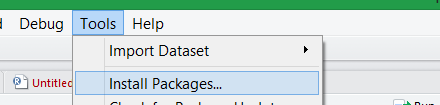
\includegraphics[width=0.5\textwidth]{images/debug}
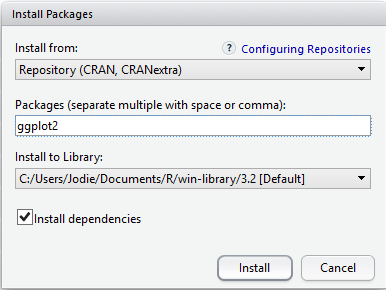
\includegraphics[width=.4\textwidth]{images/installpackage}

Or (and this would be my preferred method) type the command:
\begin{Verbatim}[label=Install package]
install.packages("ggplot2")
\end{Verbatim}
To load that library into your working session type:
\begin{Verbatim}[label=load package]
load("ggplot2") # quotes not necessary
\end{Verbatim}

\end{frame}
%%%%%%%%%%%%%%%%%%%%%%%%%%%%%%%%%%%%%%%%%%%%%%%%%%%%%%%%%%%%%%%%%%%%%%%%%%%%%%%%%%%%%%%%%%%%%%%%%%%%


%%%%%%%%%%%%%%%%%%%%%%%%%%%%%%%%%%%%%%%%%%%%%%%%%%%%%%%%%%%%%%%%%%%%%%%%%%%%%%%%%%%%%%%%%%%%%%%%%%%%
\begin{frame}[fragile]{Graphs for Qualitative Data: Frequency Tables}
\emph{Frequency tables} summarize the number of observations in each group.
\vfill
\begin{Verbatim}[xleftmargin=2em, xrightmargin=1.5em, frame=single, numbers=left, label=Frequency Table, framesep=0.5em]
> table(Auto$origin)
  1   2   3
245  68  79
\end{Verbatim}
\vfill
\end{frame}
%%%%%%%%%%%%%%%%%%%%%%%%%%%%%%%%%%%%%%%%%%%%%%%%%%%%%%%%%%%%%%%%%%%%%%%%%%%%%%%%%%%%%%%%%%%%%%%%%%%%


%%%%%%%%%%%%%%%%%%%%%%%%%%%%%%%%%%%%%%%%%%%%%%%%%%%%%%%%%%%%%%%%%%%%%%%%%%%%%%%%%%%%%%%%%%%%%%%%%%%%
\begin{frame}[fragile]{Graphs for Qualitative Data: Bar Charts}
\begin{multicols}{2}
\emph{Bar charts} have each group along the $x$-axis and a vertical bar with the height representing the number of observations of each group.
\vfill
Using the dataset {\tt Auto} in the ISLR package.
\vfill
\newpage
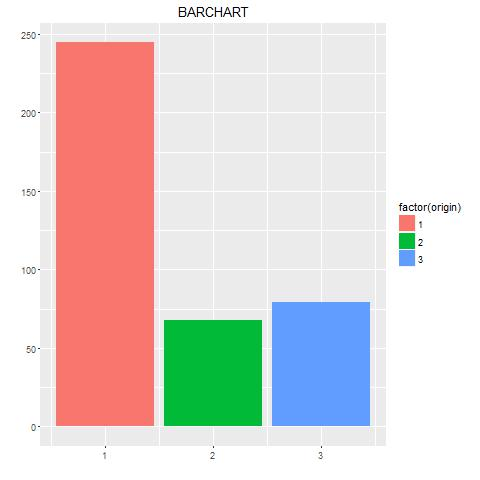
\includegraphics[width=0.4\textwidth]{images/barchart}
\end{multicols}
\begin{Verbatim}[xleftmargin=2em, xrightmargin=1.5em, frame=single, numbers=left, label=Frequency Table, framesep=0.5em]
ggplot(Auto, aes(x=origin))
+ geom_bar(aes(fill=factor(origin)))
+ xlab("") + ylab("") + ggtitle("BARCHART")
\end{Verbatim}
\end{frame}
%%%%%%%%%%%%%%%%%%%%%%%%%%%%%%%%%%%%%%%%%%%%%%%%%%%%%%%%%%%%%%%%%%%%%%%%%%%%%%%%%%%%%%%%%%%%%%%%%%%%


%%%%%%%%%%%%%%%%%%%%%%%%%%%%%%%%%%%%%%%%%%%%%%%%%%%%%%%%%%%%%%%%%%%%%%%%%%%%%%%%%%%%%%%%%%%%%%%%%%%%
\begin{frame}[fragile]{Graphs for Quantitative Data: Histogram}
\begin{multicols}{2}

A \emph{histogram} is similar to a bar chart, but the $x$-axis is divided into bins.
\vfill
The variable of interest is on the $x$-axis and the $y$-axis represents count of observations within each bin.
\vfill
Visualizes the data distribution.
\vfill
\newpage

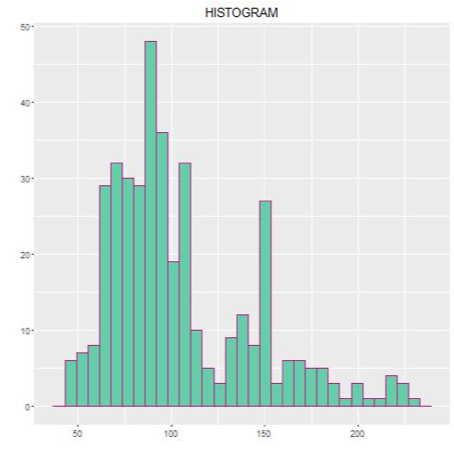
\includegraphics[width=0.4\textwidth]{images/hist}
\end{multicols}

\begin{Verbatim}[xleftmargin=.5em, xrightmargin=.5em, frame=single, label=Histogram Example, framesep=0.5em, fontsize=\small]
ggplot(Auto, aes(x=horsepower))
+ geom_histogram(color='mediumvioletred', fill='mediumaquarmarine')
+ xlab("") + ylab("") + ggtitle("HISTOGRAM")
\end{Verbatim}
\end{frame}
%%%%%%%%%%%%%%%%%%%%%%%%%%%%%%%%%%%%%%%%%%%%%%%%%%%%%%%%%%%%%%%%%%%%%%%%%%%%%%%%%%%%%%%%%%%%%%%%%%%%


%%%%%%%%%%%%%%%%%%%%%%%%%%%%%%%%%%%%%%%%%%%%%%%%%%%%%%%%%%%%%%%%%%%%%%%%%%%%%%%%%%%%%%%%%%%%%%%%%%%%
\begin{frame}[fragile]{Graphs for Quantitative Data: Boxplot}
A \emph{boxplot} is a visualization of the five number summary.
\begin{multicols}{2}
\begin{enumerate}
\item Groups along the $x$-axis.

\item Data values along the $y$-axis.

\item Lowest and highest points are the min and max of the data respectively.

\item Bottom of box is Q1 and top is Q3.

\item Median is represented as the bar inside the box.

\item Single points represent outliers.
\end{enumerate}
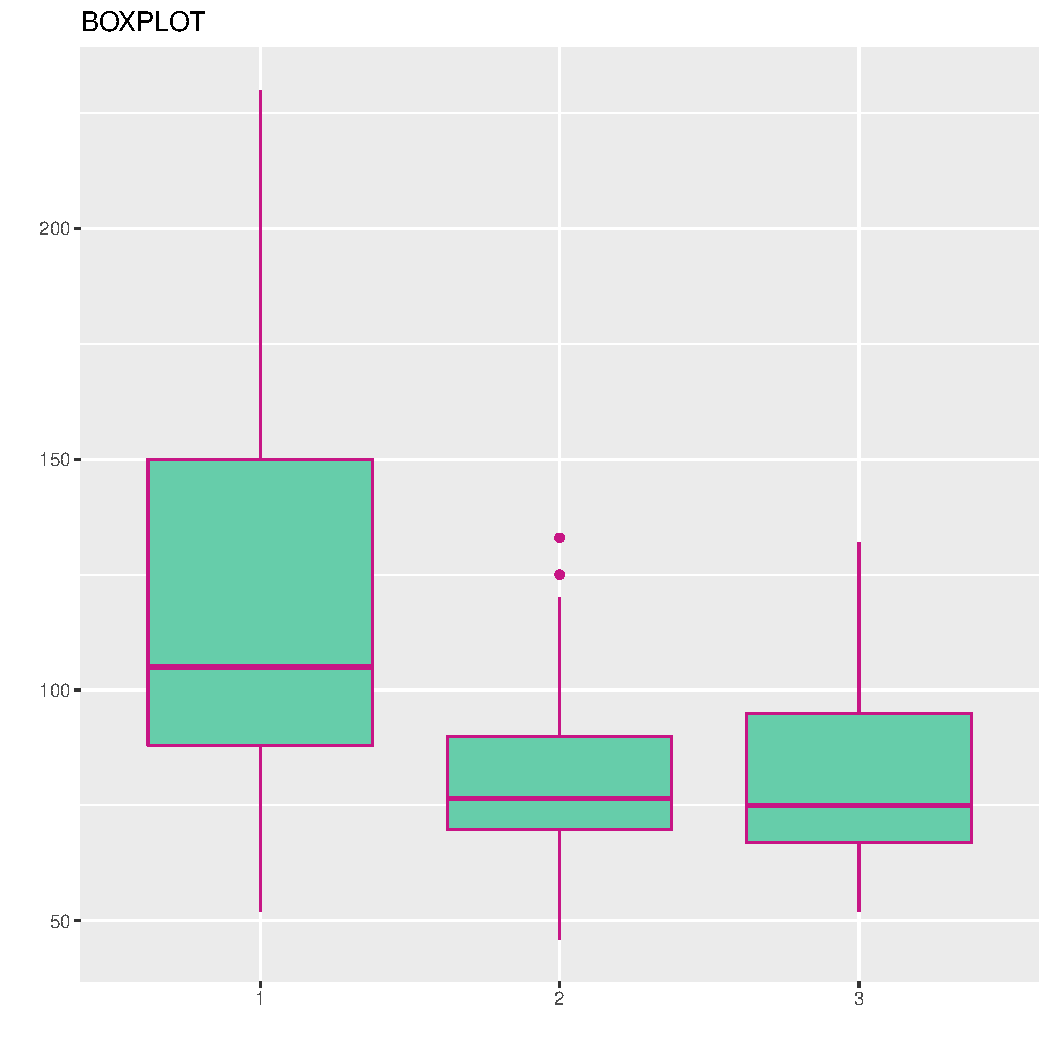
\includegraphics[width=0.4\textwidth]{images/boxplot}
\end{multicols}
\end{frame}
%%%%%%%%%%%%%%%%%%%%%%%%%%%%%%%%%%%%%%%%%%%%%%%%%%%%%%%%%%%%%%%%%%%%%%%%%%%%%%%%%%%%%%%%%%%%%%%%%%%%


%%%%%%%%%%%%%%%%%%%%%%%%%%%%%%%%%%%%%%%%%%%%%%%%%%%%%%%%%%%%%%%%%%%%%%%%%%%%%%%%%%%%%%%%%%%%%%%%%%%%
\begin{frame}[fragile]{Boxplot Example Code}
\begin{Verbatim}[xleftmargin=.5em, xrightmargin=.5em, frame=single, label=Boxplot Example, framesep=0.5em, fontsize=\small]
ggplot(Auto, aes(x=factor(origin), y=horsepower))
+ geom_boxplot(color='mediumvioletred', fill='mediumaquamarine')
+ xlab("") + ylab("") + ggtitle("BOXPLOT")
\end{Verbatim}
\end{frame}
%%%%%%%%%%%%%%%%%%%%%%%%%%%%%%%%%%%%%%%%%%%%%%%%%%%%%%%%%%%%%%%%%%%%%%%%%%%%%%%%%%%%%%%%%%%%%%%%%%%%


%%%%%%%%%%%%%%%%%%%%%%%%%%%%%%%%%%%%%%%%%%%%%%%%%%%%%%%%%%%%%%%%%%%%%%%%%%%%%%%%%%%%%%%%%%%%%%%%%%%%
\begin{frame}[fragile]{Graphs for Quantitative Data: ECDF}
\begin{multicols}{2}
An \emph{empirical cumulative distribution function (ECDF) plot} shows values along the $x$-axis and quantiles along the $y$-axis.
\vfill
Each data point is plotted along with its corresponding quantile.
\vfill
\newpage
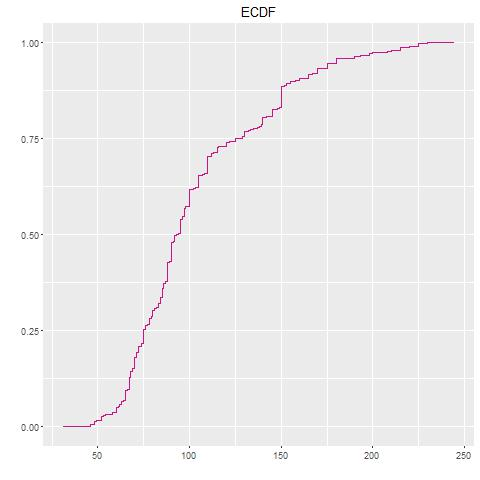
\includegraphics[width=0.4\textwidth]{images/ecdf}
\end{multicols}
\vfill
\begin{Verbatim}[xleftmargin=.5em, xrightmargin=.5em, frame=single, label=Boxplot Example, framesep=0.5em, fontsize=\small]
ggplot(Auto, aes(x=horsepower))
+ stat_ecdf(color='mediumvioletred')
+ xlab("") + ylab("") + ggtitle("ECDF")
\end{Verbatim}
\end{frame}
%%%%%%%%%%%%%%%%%%%%%%%%%%%%%%%%%%%%%%%%%%%%%%%%%%%%%%%%%%%%%%%%%%%%%%%%%%%%%%%%%%%%%%%%%%%%%%%%%%%%


%%%%%%%%%%%%%%%%%%%%%%%%%%%%%%%%%%%%%%%%%%%%%%%%%%%%%%%%%%%%%%%%%%%%%%%%%%%%%%%%%%%%%%%%%%%%%%%%%%%%
\begin{frame}[fragile]
\begin{question}
Which (if any)  of the following are true?
\begin{enumerate}
\item Bar charts and histograms will work for the same variables. \onslide<+-> \pxmark
\item Boxplots show a five number summary. \pcmark
\item Variables type does not matter, any graph can be used. \pxmark
\item Histograms can give an idea of the distribution of a variable. \pcmark
\end{enumerate}
\end{question}
\end{frame}
%%%%%%%%%%%%%%%%%%%%%%%%%%%%%%%%%%%%%%%%%%%%%%%%%%%%%%%%%%%%%%%%%%%%%%%%%%%%%%%%%%%%%%%%%%%%%%%%%%%%


%%%%%%%%%%%%%%%%%%%%%%%%%%%%%%%%%%%%%%%%%%%%%%%%%%%%%%%%%%%%%%%%%%%%%%%%%%%%%%%%%%%%%%%%%%%%%%%%%%%%
%\begin{frame}[fragile]
%\begin{question}
%\begin{enumerate}
%\item Using the car data from the \verb|data.frame| example, create a bar chart for the variable \verb|prov|.
%\item Use the cars data and create a histogram of any variable.
%\item Create a boxplot for the variable of your choice.
%\begin{enumerate}
%\item What are the median and minimum values? Can you estimate the IQR?
%\end{enumerate}
%\item Make an ECDF for the variable of your choice.
%\begin{enumerate}
%\item Recalling that Q1, median, and Q3 are the 0.25, 0.5, and 0.75th quantiles, what is yoru best guess at these values from reading off of the graphs?
%\end{enumerate}
%\end{enumerate}
%\end{question}
%\end{frame}
%%%%%%%%%%%%%%%%%%%%%%%%%%%%%%%%%%%%%%%%%%%%%%%%%%%%%%%%%%%%%%%%%%%%%%%%%%%%%%%%%%%%%%%%%%%%%%%%%%%%%


%%%%%%%%%%%%%%%%%%%%%%%%%%%%%%%%%%%%%%%%%%%%%%%%%%%%%%%%%%%%%%%%%%%%%%%%%%%%%%%%%%%%%%%%%%%%%%%%%%%%
\begin{frame}[fragile]{Confidence Intervals}
Consider the following statement
\begin{quotation}
``62\% of US college students miss a class due to excessive drinking.  The result is accurate with 1.7 percentage points 19 times out of 20.''
\end{quotation}
\vfill
Unpacking this statement:
\begin{enumerate}
\item \emph{62} is the estimated percentage.
\item \emph{1.7} is the margin of error.
\item \emph{19 times out of 20} is the stated confidence and $100\% \frac{19}{20} = 95\%$.
\end{enumerate}
\vfill
We call this a \emph{95\% confidence interval}: $(60.3,\, 63.7)$
\vfill
\end{frame}
%%%%%%%%%%%%%%%%%%%%%%%%%%%%%%%%%%%%%%%%%%%%%%%%%%%%%%%%%%%%%%%%%%%%%%%%%%%%%%%%%%%%%%%%%%%%%%%%%%%%


%%%%%%%%%%%%%%%%%%%%%%%%%%%%%%%%%%%%%%%%%%%%%%%%%%%%%%%%%%%%%%%%%%%%%%%%%%%%%%%%%%%%%%%%%%%%%%%%%%%%
\begin{frame}[fragile]
\vfill
\begin{block}{General Form of Confidence Interval}
\hfill$(\mu-me,\, \mu+me)$\hfill\hfill
\end{block}
\vfill
Interpretation of a 95\% confidence interval: we are 95\% confident that the interval will contain the true value of the parameter.
\vfill
\end{frame}
%%%%%%%%%%%%%%%%%%%%%%%%%%%%%%%%%%%%%%%%%%%%%%%%%%%%%%%%%%%%%%%%%%%%%%%%%%%%%%%%%%%%%%%%%%%%%%%%%%%%


%%%%%%%%%%%%%%%%%%%%%%%%%%%%%%%%%%%%%%%%%%%%%%%%%%%%%%%%%%%%%%%%%%%%%%%%%%%%%%%%%%%%%%%%%%%%%%%%%%%%
\begin{frame}[fragile]{Hypothesis Testing}
\emph{Hypothesis testing} is used to determine if a relationship exists between two sets of data and make decisions/conclusions about that relationship.
\vfill
\emph{Hypothesis testing is useful for}
\begin{enumerate}
\item \emph{business} in determining effectiveness of marketing, identifying customer buying properties, online advertising optimization.
\item \emph{science and social science} in determining if data sets match a model, understanding scientific process based on collected data values, analysis of study data.
\end{enumerate}
\vfill
\end{frame}
%%%%%%%%%%%%%%%%%%%%%%%%%%%%%%%%%%%%%%%%%%%%%%%%%%%%%%%%%%%%%%%%%%%%%%%%%%%%%%%%%%%%%%%%%%%%%%%%%%%%


%%%%%%%%%%%%%%%%%%%%%%%%%%%%%%%%%%%%%%%%%%%%%%%%%%%%%%%%%%%%%%%%%%%%%%%%%%%%%%%%%%%%%%%%%%%%%%%%%%%%
\begin{frame}[fragile]{Probability Distribution Functions}
\begin{description}
\item[\texttt rnorm] Random Normal variables.
\item[\texttt dnorm] Evaluate normal probability density/
\item[\texttt pnorm] 
\item[\texttt qnorm] Default distribution is ${\rm mean}=0$ and ${\rm sd}=1$.
\item[\texttt d] Density.
\item[\texttt r] Random number generation.
\item[\texttt p] Cumulative distribution.
\item[\texttt q] Quantile function.
\end{description}
\end{frame}
%%%%%%%%%%%%%%%%%%%%%%%%%%%%%%%%%%%%%%%%%%%%%%%%%%%%%%%%%%%%%%%%%%%%%%%%%%%%%%%%%%%%%%%%%%%%%%%%%%%%


%%%%%%%%%%%%%%%%%%%%%%%%%%%%%%%%%%%%%%%%%%%%%%%%%%%%%%%%%%%%%%%%%%%%%%%%%%%%%%%%%%%%%%%%%%%%%%%%%%%%
\begin{frame}[fragile]{Hypothesis Testing Steps}
\begin{enumerate}
\item Declare hypotheses statement and null hypothesis.
\item Decide on a test statistic.
\item Use P-value and/or confidence interval to make decision/conclusion.
\begin{enumerate}
\item A p-value of 0.05 ``signifies that if the null hypothesis is true, and all other assumptions made are valid, there is a 5\% chance of obtaining a result at least as extreme as the one observed.''
\end{enumerate}
\item Data is used as evidence.  Perform a test in order to make a decision:  reject the null hypothesis or fail to reject the null hypothesis.
\end{enumerate}
\vfill
Note: We cannot \emph{prove} that the null hypothesis is true or false. We can only show that there is evidence to suggest one conclusion or another. 
\end{frame}
%%%%%%%%%%%%%%%%%%%%%%%%%%%%%%%%%%%%%%%%%%%%%%%%%%%%%%%%%%%%%%%%%%%%%%%%%%%%%%%%%%%%%%%%%%%%%%%%%%%%

%%%%%%%%%%%%%%%%%%%%%%%%%%%%%%%%%%%%%%%%%%%%%%%%%%%%%%%%%%%%%%%%%%%%%%%%%%%%%%%%%%%%%%%%%%%%%%%%%%%%
\begin{frame}[fragile]{Assumptions}
\vfill
There are assumptions that need to be met before performing statistical tests.
\vfill
For the one sample:
\begin{enumerate}
\item Population of interest is normally distributed.
\item Independent random samples are taken.
\end{enumerate}
\vfill
For the two sample case:
\begin{enumerate}
\item The two samples are independent.
\item Populations of interest are normally distributed.
\end{enumerate}
\vfill
\end{frame}
%%%%%%%%%%%%%%%%%%%%%%%%%%%%%%%%%%%%%%%%%%%%%%%%%%%%%%%%%%%%%%%%%%%%%%%%%%%%%%%%%%%%%%%%%%%%%%%%%%%%


%%%%%%%%%%%%%%%%%%%%%%%%%%%%%%%%%%%%%%%%%%%%%%%%%%%%%%%%%%%%%%%%%%%%%%%%%%%%%%%%%%%%%%%%%%%%%%%%%%%%
\begin{frame}[fragile]{One Sample Test}
\vfill
A \emph{one sample test} is used when a sample is compared to a model or known population/estimate.
\vfill
As an example, using the car data test if the average mileage is different than 10km/L.
\vfill
\end{frame}
%%%%%%%%%%%%%%%%%%%%%%%%%%%%%%%%%%%%%%%%%%%%%%%%%%%%%%%%%%%%%%%%%%%%%%%%%%%%%%%%%%%%%%%%%%%%%%%%%%%%


%%%%%%%%%%%%%%%%%%%%%%%%%%%%%%%%%%%%%%%%%%%%%%%%%%%%%%%%%%%%%%%%%%%%%%%%%%%%%%%%%%%%%%%%%%%%%%%%%%%%
\begin{frame}[fragile]{One Sample Test: Hypotheses Statements}
Null hypothesis ($H_0$) always contains a statement of no change ($=$).
\vfill
Alternatively hypothesis ($H_A$) can be one sided ($<$ or $>$) or two sided ($\neq$).
\begin{enumerate}
\item $H_0$: $\mu = \verb|test_number|$,
\item $H_A$: $\mu \neq \verb|test_number|$.
\end{enumerate}
\vfill
Car mileage example
\begin{enumerate}
\item $H_0$: $\mu = \verb|10|$,
\item $H_A$: $\mu \neq \verb|10|$.
\end{enumerate}
\vfill
\end{frame}
%%%%%%%%%%%%%%%%%%%%%%%%%%%%%%%%%%%%%%%%%%%%%%%%%%%%%%%%%%%%%%%%%%%%%%%%%%%%%%%%%%%%%%%%%%%%%%%%%%%%


%%%%%%%%%%%%%%%%%%%%%%%%%%%%%%%%%%%%%%%%%%%%%%%%%%%%%%%%%%%%%%%%%%%%%%%%%%%%%%%%%%%%%%%%%%%%%%%%%%%%
\begin{frame}[fragile]{One Sample Test: Calculate Test Statistic}
\vfill
For the one sample test the $t$-test statistic is calculated as:
$$t = \dfrac{\bar y - \mu_0}{\dfrac{s}{\sqrt n}}$$
\vfill
$\overline y$ is a sample mean, $s$ is sample standard deviation, $n$ is sample size, $\mu_0$ is hypothesized mean value
\vfill
\begin{Verbatim}[xleftmargin=2em, xrightmargin=1.5em, frame=single, label=R code, framesep=0.5em]
car_data <- read.csv("car_data.csv")
t.test(x=car_data$km.L,
       alternative=c("two.sided"), mu=10)
\end{Verbatim}
\end{frame}
%%%%%%%%%%%%%%%%%%%%%%%%%%%%%%%%%%%%%%%%%%%%%%%%%%%%%%%%%%%%%%%%%%%%%%%%%%%%%%%%%%%%%%%%%%%%%%%%%%%%


%%%%%%%%%%%%%%%%%%%%%%%%%%%%%%%%%%%%%%%%%%%%%%%%%%%%%%%%%%%%%%%%%%%%%%%%%%%%%%%%%%%%%%%%%%%%%%%%%%%%
\begin{frame}[fragile]{One Sample Test: Decision and Conclusion (using $P$-value)}
\vfill
If $p{\rm-value} > 0.05$, the probability of seeing a sample mean more extreme is not that unlikely.
\begin{enumerate}
\item Fail to reject the null hypothesis.
\item There is no evidence to suggest that the mean value is less than, greater than, or different than the test value.
\end{enumerate}
\vfill
If $p{\rm-value} < 0.05$,
\begin{enumerate}
\item Reject the null hypothesis.
\item There is statistically significant evidence to suggest that the mean value is less than that, greater than, or different than the test value.
\end{enumerate}
\vfill
\end{frame}
%%%%%%%%%%%%%%%%%%%%%%%%%%%%%%%%%%%%%%%%%%%%%%%%%%%%%%%%%%%%%%%%%%%%%%%%%%%%%%%%%%%%%%%%%%%%%%%%%%%%


%%%%%%%%%%%%%%%%%%%%%%%%%%%%%%%%%%%%%%%%%%%%%%%%%%%%%%%%%%%%%%%%%%%%%%%%%%%%%%%%%%%%%%%%%%%%%%%%%%%%
\begin{frame}[fragile]{One Sample Test: Decision and Conclusions (using $P$-value)}
\begin{Verbatim}[xleftmargin=2em, xrightmargin=1.5em, frame=single, label=R code, framesep=0.5em, fontsize=\small, commandchars=\\\{\}]
> t.test(x=car_data$km.L, alternative=c("two.sided"),mu=10)
            
            One Sample t-test
            
data: car_data$km.L
t = 1.608, df = 29, \emph{p-value = 0.1187}
alternative hypothesis: true mean is not equal to 10
95 percent confidence interval:
    9.90338  10.80729
sample estimates:
mean of x
  10.35533
\end{Verbatim}
\end{frame}
%%%%%%%%%%%%%%%%%%%%%%%%%%%%%%%%%%%%%%%%%%%%%%%%%%%%%%%%%%%%%%%%%%%%%%%%%%%%%%%%%%%%%%%%%%%%%%%%%%%%


%%%%%%%%%%%%%%%%%%%%%%%%%%%%%%%%%%%%%%%%%%%%%%%%%%%%%%%%%%%%%%%%%%%%%%%%%%%%%%%%%%%%%%%%%%%%%%%%%%%%
\begin{frame}[fragile]{One Sample Test: Decision and Conclusions (using $P$-value)}
\vfill
$P$-value $=0.1187 > 0.05 \implies \text{ fail to reject the null hypothesis}$.
\vfill
There is no evidence to suggest that the mean mileage is no 10 km/L.
\vfill
Note: Unable to claim that either the null or alternative hypothesis is true.  Can only reject or fail to reject the null hypothesis.
\vfill
\end{frame}
%%%%%%%%%%%%%%%%%%%%%%%%%%%%%%%%%%%%%%%%%%%%%%%%%%%%%%%%%%%%%%%%%%%%%%%%%%%%%%%%%%%%%%%%%%%%%%%%%%%%


%%%%%%%%%%%%%%%%%%%%%%%%%%%%%%%%%%%%%%%%%%%%%%%%%%%%%%%%%%%%%%%%%%%%%%%%%%%%%%%%%%%%%%%%%%%%%%%%%%%%
\begin{frame}[fragile]{One Sample Test: Decision and Conclusions (using CI)}\small
\begin{Verbatim}[xleftmargin=2em, xrightmargin=1.5em, frame=single, label=R code, framesep=0.5em, fontsize=\footnotesize, commandchars=\\\{\}]
> t.test(x=car_data$km.L, alternative=c("two.sided"),mu=10)
            One Sample t-test
data: car_data$km.L
t = 1.608, df = 29, p-value = 0.1187
alternative hypothesis: true mean is not equal to 10
\emph{95 percent confidence interval:}
\emph{    9.90338  10.80729}
sample estimates:
mean of x
  10.35533
\end{Verbatim}
Can also make a conclusion (reject or fail to reject) based on the confidence interval. We are 95\% confident that the true mean mileage of the car lies within those bounds. 
\vfill
Since 10 km/L is within those bounds, fail to reject the null hypothesis.
\vfill
\end{frame}
%%%%%%%%%%%%%%%%%%%%%%%%%%%%%%%%%%%%%%%%%%%%%%%%%%%%%%%%%%%%%%%%%%%%%%%%%%%%%%%%%%%%%%%%%%%%%%%%%%%%


%%%%%%%%%%%%%%%%%%%%%%%%%%%%%%%%%%%%%%%%%%%%%%%%%%%%%%%%%%%%%%%%%%%%%%%%%%%%%%%%%%%%%%%%%%%%%%%%%%%%
\begin{frame}[fragile]{Two Sample Unpaired}
\vfill
An unpaired (independent) \emph{two sample test} compares two independent samples to determine if there is a difference between the groups.
\vfill
\begin{example}
\begin{enumerate}
\item Compare effectiveness of two different drugs tested on two sets of patients.\\
\item Experiment versus control samples.
\end{enumerate}
\end{example}
\vfill
\end{frame}
%%%%%%%%%%%%%%%%%%%%%%%%%%%%%%%%%%%%%%%%%%%%%%%%%%%%%%%%%%%%%%%%%%%%%%%%%%%%%%%%%%%%%%%%%%%%%%%%%%%%


%%%%%%%%%%%%%%%%%%%%%%%%%%%%%%%%%%%%%%%%%%%%%%%%%%%%%%%%%%%%%%%%%%%%%%%%%%%%%%%%%%%%%%%%%%%%%%%%%%%%
\begin{frame}[fragile]{Two Sample Unpaired Example
Hypothesis Statement}
Using the \verb|beaver2| dataset in R, test the hypothesis that there is no difference between the mean active temperature and the mean non-active temperatures.
\begin{align*}
H_0 : \mu_1 = \mu_2 \to \mu_1 -\mu_2 = 0 \\
H_A : \mu1 \neq \mu_2 \to \mu_1 - \mu_2 \neq 0
\end{align*}
\end{frame}
%%%%%%%%%%%%%%%%%%%%%%%%%%%%%%%%%%%%%%%%%%%%%%%%%%%%%%%%%%%%%%%%%%%%%%%%%%%%%%%%%%%%%%%%%%%%%%%%%%%%


%%%%%%%%%%%%%%%%%%%%%%%%%%%%%%%%%%%%%%%%%%%%%%%%%%%%%%%%%%%%%%%%%%%%%%%%%%%%%%%%%%%%%%%%%%%%%%%%%%%%
\begin{frame}[fragile]{Two Sample Unpaired Example Test Statistic}
\vfill
Use $t$-test statistics.
\vfill
\begin{Verbatim}[xleftmargin=2em, xrightmargin=1.5em, frame=single, numbers=left, label=Using P-value, framesep=0.5em, commandchars=\\\{\}]
# Need to set active to be a factor first.
beaver2$activ = as.factor(beaver2$activ)
# Perform unpaired test
t.test(temp{~}activ, data=beaver2,
       alternative=c("two.sided"), mu=0,
       paired=FALSE)
\end{Verbatim}
\vfill
\end{frame}
%%%%%%%%%%%%%%%%%%%%%%%%%%%%%%%%%%%%%%%%%%%%%%%%%%%%%%%%%%%%%%%%%%%%%%%%%%%%%%%%%%%%%%%%%%%%%%%%%%%%


%%%%%%%%%%%%%%%%%%%%%%%%%%%%%%%%%%%%%%%%%%%%%%%%%%%%%%%%%%%%%%%%%%%%%%%%%%%%%%%%%%%%%%%%%%%%%%%%%%%%
\begin{frame}[fragile]{Two Sample Unpaired Example Decision and Conclusions}
\begin{Verbatim}[xleftmargin=2em, xrightmargin=1.5em, frame=single, label=Using CI-value, framesep=0.5em, commandchars=\\\{\}, fontsize=\footnotesize]
> t.text(temp-activ, data=beaver2, alternative=c("two.sided"), mu=0,
paired=FALSE)
        welch Two Sample t-test
data:    temp by activ
t = -18.548,  df = 80.852, \emph{p-value < 2.2e-16}
alternative hypothesis: true difference in means is not equal to 0
95 percent condifence interval:
  -0.8927106  -0.7197342
sample estimates:
mean in group 0 mean in group 1
        37.09684        37.90306
\end{Verbatim}
The p-value $<<$ 0.05.
\vfill
Reject the null hypothesis. There is vert strong evidence to suggest that there is a difference between active and non-active temperatures. 
\end{frame}
%%%%%%%%%%%%%%%%%%%%%%%%%%%%%%%%%%%%%%%%%%%%%%%%%%%%%%%%%%%%%%%%%%%%%%%%%%%%%%%%%%%%%%%%%%%%%%%%%%%%

\begin{frame}
The two sample case tests a DIFFERENCE between the groups $(\mu_1 - \mu_2 \neq 0)$. \\[0.2in]
The CI stated on the previous slide is the CI for the difference, $\mu_1 - \mu_2$\\[0.2in]
We reject the null hypothesis because 0 is not contained in the interval. \\[0.2in]
If 0 was contained we would fail to reject the null hypothesis.
%
\end{frame}

%%%%%%%%%%%%%%%%%%%%%%%%%%%%%%%%%%%%%%%%%%%%%%%%%%%%%%%%%%%%%%%%%%%%%%%%%%%%%%%%%%%%%%%%%%%%%%%%%%%%
\begin{frame}[fragile]{Two Sample Paired Test}
A \emph{paired (dependent) two sample test} compares two dependent samples to see if there is a difference between the groups.
\begin{enumerate}
\item This test typically uses multiple measurements on one subject.
\item Also called a "repeated measures" test.
\end{enumerate}
\vfill
\begin{examples}
\begin{enumerate}
\item Affect of treatment on a patient (before and after)
\item Apply something to test subjects to see if there is an effect
\item Car example: Do cars get better mileage with different grades of gasoline?
\end{enumerate}
\end{examples}

\end{frame}
%%%%%%%%%%%%%%%%%%%%%%%%%%%%%%%%%%%%%%%%%%%%%%%%%%%%%%%%%%%%%%%%%%%%%%%%%%%%%%%%%%%%%%%%%%%%%%%%%%%%


%%%%%%%%%%%%%%%%%%%%%%%%%%%%%%%%%%%%%%%%%%%%%%%%%%%%%%%%%%%%%%%%%%%%%%%%%%%%%%%%%%%%%%%%%%%%%%%%%%%%
\begin{frame}[fragile]{Two Sample Paired Test Example Hypothesis Statement}
\vfill
The \verb|ahtlete.csv| dataset contains data on ten athletes and their speeds for the 100m dash before training (Training = 0) and after (Training = 1).
\vfill
Test the hypothesis that the training has no effect on the times of the athletes.  Test to see if the mean of the difference is different than 0.
\begin{align*}
H_0 &: d = 0\\
H_A &: d \neq 0
\end{align*}
\vfill
\end{frame}
%%%%%%%%%%%%%%%%%%%%%%%%%%%%%%%%%%%%%%%%%%%%%%%%%%%%%%%%%%%%%%%%%%%%%%%%%%%%%%%%%%%%%%%%%%%%%%%%%%%%


%%%%%%%%%%%%%%%%%%%%%%%%%%%%%%%%%%%%%%%%%%%%%%%%%%%%%%%%%%%%%%%%%%%%%%%%%%%%%%%%%%%%%%%%%%%%%%%%%%%%
\begin{frame}[fragile]{Two Sample Paired Test Example Test Statistic -- R Code}
\begin{Verbatim}[xleftmargin=2em, xrightmargin=1.5em, frame=single, label=Using CI-value, framesep=0.5em, commandchars=\\\{\}, fontsize=\small]
# Read the data
athlete = read.csv("athlete.csv", header=TRUE)

# Perform paired test
t.test(Time~Training, data=athlete, 
  alternative=c("two.sided"), my=0, paired=TRUE)
\end{Verbatim}
\end{frame}
%%%%%%%%%%%%%%%%%%%%%%%%%%%%%%%%%%%%%%%%%%%%%%%%%%%%%%%%%%%%%%%%%%%%%%%%%%%%%%%%%%%%%%%%%%%%%%%%%%%%


%%%%%%%%%%%%%%%%%%%%%%%%%%%%%%%%%%%%%%%%%%%%%%%%%%%%%%%%%%%%%%%%%%%%%%%%%%%%%%%%%%%%%%%%%%%%%%%%%%%%
\begin{frame}[fragile]{Two Sample Paired Test Example  Decision and Conclusion}
\begin{Verbatim}[xleftmargin=2em, xrightmargin=1.5em, frame=single, label=Using P-value, framesep=0.5em, commandchars=\\\{\}, fontsize=\footnotesize]
> t.test(Time~Training, data=athlete, alternative=c("two.sided"),
  mu=0, paired=TRUE)
        Paired t-test
data:    Time by Training
t = -0.12031, df = 9, \emph{p-value = 0.9069}
alternative hypothesis: true difference in means is not equal to 0
95 percent confidence interval:
-0.5544647  0.4984647
sample estimates:
mean of the differences
                 -0.028
\end{Verbatim}
The $p{\rm -value}>>0.05$.
\vfill
Fail to reject the null hypothesis.  There is no evidence to suggest that there is a difference between pre and post training times.
\end{frame}
%%%%%%%%%%%%%%%%%%%%%%%%%%%%%%%%%%%%%%%%%%%%%%%%%%%%%%%%%%%%%%%%%%%%%%%%%%%%%%%%%%%%%%%%%%%%%%%%%%%%


%%%%%%%%%%%%%%%%%%%%%%%%%%%%%%%%%%%%%%%%%%%%%%%%%%%%%%%%%%%%%%%%%%%%%%%%%%%%%%%%%%%%%%%%%%%%%%%%%%%%
\begin{frame}[fragile]{Two Sample Paired Test Example Decision and Conclusion}
\begin{Verbatim}[xleftmargin=2em, xrightmargin=1.5em, frame=single, label=Using CI, framesep=0.5em, commandchars=\\\{\}, fontsize=\footnotesize]
> t.test(Time-Training, data=athlete, alternative=c("two.sided"), 
  mu=0, paired=TRUE)
        Paired t-test
data:    Time by training
t = -0.12031,  df = 9,  p-values = 0.9069
alternative hypothesis true difference in means is not equal to 0
-0.5544647   0.4984647
sample estimates:
mean of the differences
                 -0.028
\end{Verbatim}
The two sample case tests for a difference between the groups ($d \neq 0$).  The CI is for the difference.
\vfill
Fail to reject the null hypothesis because 0 is contained in the confidence interval.
\end{frame}
%%%%%%%%%%%%%%%%%%%%%%%%%%%%%%%%%%%%%%%%%%%%%%%%%%%%%%%%%%%%%%%%%%%%%%%%%%%%%%%%%%%%%%%%%%%%%%%%%%%%


%%%%%%%%%%%%%%%%%%%%%%%%%%%%%%%%%%%%%%%%%%%%%%%%%%%%%%%%%%%%%%%%%%%%%%%%%%%%%%%%%%%%%%%%%%%%%%%%%%%%
\begin{frame}[fragile]
\begin{question}
Which (if any) of the following are true?
\begin{enumerate}
\item Paired and unpaired $t$-tests are the same thing. \onslide<+-> \pxmark
\item Confidence intervals can be of any level of confidence (not just 95\%). \pcmark
\item Confidence intervals can be used to make a conclusion about a hypothesis test. \pcmark
\item Confidence intervals can be used to prove that the null hypothesis is false. \pxmark
\end{enumerate}
\end{question}
\end{frame}
%%%%%%%%%%%%%%%%%%%%%%%%%%%%%%%%%%%%%%%%%%%%%%%%%%%%%%%%%%%%%%%%%%%%%%%%%%%%%%%%%%%%%%%%%%%%%%%%%%%%


%%%%%%%%%%%%%%%%%%%%%%%%%%%%%%%%%%%%%%%%%%%%%%%%%%%%%%%%%%%%%%%%%%%%%%%%%%%%%%%%%%%%%%%%%%%%%%%%%%%%
\begin{frame}[fragile]
\begin{question}
Which (if any) of the following are true?
\begin{enumerate}
\item Unpaired t-tests test the difference between two means $\mu_1$ and $\mu_2$.
\item Paired t-tests can be used to compare the difference between two measurements on the same subject.
\item In both the paired and unpaired two sample cases, a confidence interval containing 0 would result in a decision of: fail to reject the null hypothesis.
\item  In the one sample $t$-test, a confidence interval containing 0 would result in a decision of: fail to reject the null hypothesis.
\end{enumerate}
\end{question}
\end{frame}
%%%%%%%%%%%%%%%%%%%%%%%%%%%%%%%%%%%%%%%%%%%%%%%%%%%%%%%%%%%%%%%%%%%%%%%%%%%%%%%%%%%%%%%%%%%%%%%%%%%%


%%%%%%%%%%%%%%%%%%%%%%%%%%%%%%%%%%%%%%%%%%%%%%%%%%%%%%%%%%%%%%%%%%%%%%%%%%%%%%%%%%%%%%%%%%%%%%%%%%%%
\begin{frame}[fragile]\small
\begin{question}
Which is the most appropriate test for each of the following?
\begin{enumerate}
\item Is the average student mark in courses 70\%?  \onslide<+->{one sample}
\item Does a student's mark improve after studying?  \onslide<+->{two sample paired (same student)}
\item Has the average student height increased since 1990?  \onslide<+->{two sample unpaired (two distinct student populations)}
\end{enumerate}
\end{question}
\end{frame}
%%%%%%%%%%%%%%%%%%%%%%%%%%%%%%%%%%%%%%%%%%%%%%%%%%%%%%%%%%%%%%%%%%%%%%%%%%%%%%%%%%%%%%%%%%%%%%%%%%%%


%%%%%%%%%%%%%%%%%%%%%%%%%%%%%%%%%%%%%%%%%%%%%%%%%%%%%%%%%%%%%%%%%%%%%%%%%%%%%%%%%%%%%%%%%%%%%%%%%%%%
\begin{frame}[fragile]\small
\begin{question}
Which is the most appropriate test for each of the following?
\begin{enumerate}
\item Does radiation reduce the size of tumours when used to treat patients?  \onslide<+->{two sample paired (same patient), although could argue against control/experiment groups in which case two sample unpaired}
\item Is aspirin more effective than Tylenol for treating headaches?  \onslide<+->{ two sample unpaired }
\item Are college graduates better than high school graduates at standardized tests?   \onslide<+->{ two sample unpaired }
\end{enumerate}
\end{question}
\end{frame}
%%%%%%%%%%%%%%%%%%%%%%%%%%%%%%%%%%%%%%%%%%%%%%%%%%%%%%%%%%%%%%%%%%%%%%%%%%%%%%%%%%%%%%%%%%%%%%%%%%%%


%%%%%%%%%%%%%%%%%%%%%%%%%%%%%%%%%%%%%%%%%%%%%%%%%%%%%%%%%%%%%%%%%%%%%%%%%%%%%%%%%%%%%%%%%%%%%%%%%%%%
\begin{frame}[fragile]
\begin{question}
Using the car data, test the hypothesis that the mean distance at each fill up is less than 450km.
\end{question}
\vfill
\begin{question}
Use the car data to see if the mean distance for Alberta fill ups is different than the mean distance for B.C fill ups.
\end{question}
\pause
\pause
\verb|t.test(x = car_data Distance, alternative=c("less"), mu=450)|
\pause
\verb|t.test(Distance~prov, data=car_data, alternative=c("two.sided"), mu=0, paired =FALSE)|
\end{frame}
%%%%%%%%%%%%%%%%%%%%%%%%%%%%%%%%%%%%%%%%%%%%%%%%%%%%%%%%%%%%%%%%%%%%%%%%%%%%%%%%%%%%%%%%%%%%%%%%%%%%


%%%%%%%%%%%%%%%%%%%%%%%%%%%%%%%%%%%%%%%%%%%%%%%%%%%%%%%%%%%%%%%%%%%%%%%%%%%%%%%%%%%%%%%%%%%%%%%%%%%%
\begin{frame}[fragile]{Linear models in R}
\vfill
A linear model is an equation that relates a response variable ($y$) to some explanatory variables ($x$'s).  The general form of the model is:
$$y = b_0 + b_1x_1 + b_2x_2 + \cdots + b_nx_n$$
\vfill
Not all of the data points can fall on this line so the full equation is
$$y_i = b_0 + b_1 x_{1i} + b_2x_{2i} + \cdot + b_nx_{bi} + \varepsilon_i$$
\vfill
Where $\varepsilon_i$ denotes the error term associated with observation $i$.
\vfill
\end{frame}
%%%%%%%%%%%%%%%%%%%%%%%%%%%%%%%%%%%%%%%%%%%%%%%%%%%%%%%%%%%%%%%%%%%%%%%%%%%%%%%%%%%%%%%%%%%%%%%%%%%%

%%%%%%%%%%%%%%%%%%%%%%%%%%%%%%%%%%%%%%%%%%%%%%%%%%%%%%%%%%%%%%%%%%%%%%%%%%%%%%%%%%%%%%%%%%%%%%%%%%%%
\begin{frame}[fragile]{Linear models in R}
We are assuming
\begin{enumerate}
\item Residuals are independent.
\item Residuals are normally distributed.
\item Residuals have a mean of 0 for all $X$.
\item Residuals have constant variance.
\end{enumerate}
\end{frame}
%%%%%%%%%%%%%%%%%%%%%%%%%%%%%%%%%%%%%%%%%%%%%%%%%%%%%%%%%%%%%%%%%%%%%%%%%%%%%%%%%%%%%%%%%%%%%%%%%%%%


%%%%%%%%%%%%%%%%%%%%%%%%%%%%%%%%%%%%%%%%%%%%%%%%%%%%%%%%%%%%%%%%%%%%%%%%%%%%%%%%%%%%%%%%%%%%%%%%%%%%
\begin{frame}[fragile]{Fitting a Linear Model}
\begin{Verbatim}[xleftmargin=2em, xrightmargin=1.5em, frame=single, label=Using P-value, framesep=0.5em, commandchars=\\\{\}, fontsize=\small]
> lm(km.L~Litres+Distance, data=car_data)
> model

call:
lm(formula = km.L ~ Litres + Distance, data = car_data)

Coefficients:
(Intercept)        Litres        Distance
  10.35447       -0.33295         0.03251
\end{Verbatim}
The formula can be then be created using the values stored in \verb|model$coefficients|

\verb|Km.L = 10.35447 -0.33295*Litres + 0.03251*Distance|
\end{frame}
%%%%%%%%%%%%%%%%%%%%%%%%%%%%%%%%%%%%%%%%%%%%%%%%%%%%%%%%%%%%%%%%%%%%%%%%%%%%%%%%%%%%%%%%%%%%%%%%%%%%


%%%%%%%%%%%%%%%%%%%%%%%%%%%%%%%%%%%%%%%%%%%%%%%%%%%%%%%%%%%%%%%%%%%%%%%%%%%%%%%%%%%%%%%%%%%%%%%%%%%%
\begin{frame}[fragile]{Conclusion}
\begin{enumerate}
\item R is a free and open source programming language for statistical computing and graphics.
\item R contains many useful features for data analysis including data structures such as vectors and data frames that make it easy to perform statistical analysis and visualization.
\item R is often used for hypothesis testing and understanding how to properly setup and interpret a test is an important skill.
\end{enumerate}
\end{frame}
%%%%%%%%%%%%%%%%%%%%%%%%%%%%%%%%%%%%%%%%%%%%%%%%%%%%%%%%%%%%%%%%%%%%%%%%%%%%%%%%%%%%%%%%%%%%%%%%%%%%



\end{document}
%%%%%%%%%%%%%%%%%%%%%%%%%%%%%%%%%%%%%%%%%%%%%%%%%%%%%%%%%%%%%%%%%%%%%%%%%%%%%%%%%%%%%%%%%%%%%%%%%%%%
